\documentclass[11pt]{article}
\usepackage{booktabs,xcolor,pgfplots}
\pgfplotsset{compat=1.18}
\begin{document}
\section*{Test 4: Warm-Start Effectiveness}

\subsection*{Cache Statistics}
\begin{tabular}{lr}
\toprule
Metric & Value \\\midrule
Total points & 24 \\
Cache hits & 12 (50.0\%) \\
Cache misses & 12 \\
Fallbacks & 0 \\
\midrule
Total time (cold) & 29.5657 s \\
Total time (warm) & 29.0307 s \\
\textbf{Speedup} & \textbf{1.02\texttimes} \\
\bottomrule\end{tabular}

\subsection*{Time per Point}
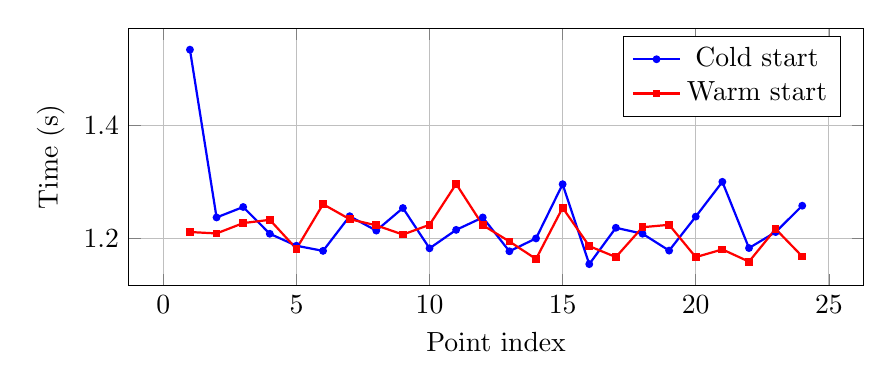
\begin{tikzpicture}
\begin{axis}[
    xlabel={Point index},
    ylabel={Time (s)},
    legend pos=north east,
    width=0.9\textwidth,
    height=0.4\textwidth,
    grid=major,
]

\addplot[blue, mark=*, thick, mark size=1pt] coordinates {(1, 1.5343) (2, 1.2371) (3, 1.2556) (4, 1.2082) (5, 1.1870) (6, 1.1779) (7, 1.2393) (8, 1.2138) (9, 1.2538) (10, 1.1824) (11, 1.2151) (12, 1.2371) (13, 1.1772) (14, 1.2000) (15, 1.2960) (16, 1.1544) (17, 1.2188) (18, 1.2083) (19, 1.1784) (20, 1.2386) (21, 1.3002) (22, 1.1829) (23, 1.2112) (24, 1.2579) };
\addlegendentry{Cold start}
\addplot[red, mark=square*, thick, mark size=1pt] coordinates {(1, 1.2113) (2, 1.2088) (3, 1.2271) (4, 1.2329) (5, 1.1816) (6, 1.2606) (7, 1.2341) (8, 1.2231) (9, 1.2068) (10, 1.2241) (11, 1.2965) (12, 1.2234) (13, 1.1946) (14, 1.1635) (15, 1.2543) (16, 1.1863) (17, 1.1669) (18, 1.2198) (19, 1.2241) (20, 1.1668) (21, 1.1805) (22, 1.1588) (23, 1.2167) (24, 1.1681) };
\addlegendentry{Warm start}
\end{axis}
\end{tikzpicture}

\subsection*{Threshold Sensitivity}
\begin{tabular}{rrrr}
\toprule
Threshold & Speedup & Hit Rate & Fallbacks \\\midrule
0.010 & 0.94\texttimes & 0.0\% & 0 \\
0.020 & 1.01\texttimes & 0.0\% & 0 \\
0.050 & 1.02\texttimes & 50.0\% & 0 \\
0.100 & 1.01\texttimes & 66.7\% & 0 \\
0.200 & 1.02\texttimes & 83.3\% & 0 \\
\bottomrule\end{tabular}

\end{document}
